В данной главе рассматривается задача выбора структуры модели глубокого обучения. Предлагается ввести вероятностные предположения о распределениях параметров и структуры модели. 
Проводится градиентная оптимизация параметров и гиперпараметров модели на основе байесовского вариационного вывода.  В качестве оптимизируемой функции для гиперпараметров модели предлагается обобщенная функция обоснованности. Показано, что данная функция позволяет проводить оптимизацию, соответствующую нескольким криетериям выбора структуры модели: методу максимального правдоподобия, последовательному увеличению и снижению сложности модели, полному перебору структуры модели, а также получению максимума вариационной оценки обоснованности модели. Решается двухуровневая задача оптимизации: на первом уровне проводится оптимизация нижней оценки обоснованности модели по вариационным параметрам модели. На втором уровне проводится оптимизация гиперпараметров модели.

\section{Вероятностная модель}
Определим априорные распределения параметров и структуры модели следующим образом.
Пусть параметры модели распределены нормально с нулевым средним:
\[
    \mathbf{w}^{i,j}_k \sim \mathcal{N}\bigl(\mathbf{0}, (\gamma^{i,j}_k\mathbf{A}^{i,j}_k)^{-1}\bigr),
\]
где $ (\mathbf{A}^{i,j}_k)^{-1}$ --- диагональная матрица. Апирорное распределение $p(\mathbf{w}|\boldsymbol{\Gamma}, \mathbf{h})$ параметров $\mathbf{w}^{i,j}_k$ зависит не только от гиперпараметров $\mathbf{A}_k^{i,j}$, но и от структурного параметра $\gamma^{i,j}_k$.

Заметим, что предлагаемое априорное распределение неоднозначно: одно и то же распределение  можно получить с различными значениями гиперпарамета $\mathbf{A}^{i,j}_k$ и структурного параметра $\gamma^{i,j}_k$. В качестве регуляризатора для матрицы $(\mathbf{A}^{i,j}_k)^{-1}$ предлагается использовать обратное гамма-распределение:
\[
    (\mathbf{A}^{i,j}_k)^{-1} \sim \text{inv-gamma}(\lambda_1,\lambda_2),
\]
где $\lambda_1,\lambda_2 \in \boldsymbol{\lambda}$ --- метапараметры оптимизации. 
Использование обратного гамма-распределения в качестве распределения гиперпараметров можно найти в~\cite{bishop,mackay}. В данной работе обратное распределение выступает как регуляризатор гиперпараметров.
Калибруя метапарамы   $\lambda_1,\lambda_2$ можно получить более сильную или более слабую регуляризацию~\cite{rvm}. Пример распределений $\text{inv-gamma}(\lambda_1,\lambda_2)$ для разных значений метапараметров $\lambda_1,\lambda_2$ изображен на Рис.~\ref{fig:inv-gamma}.

\begin{figure}
\centering
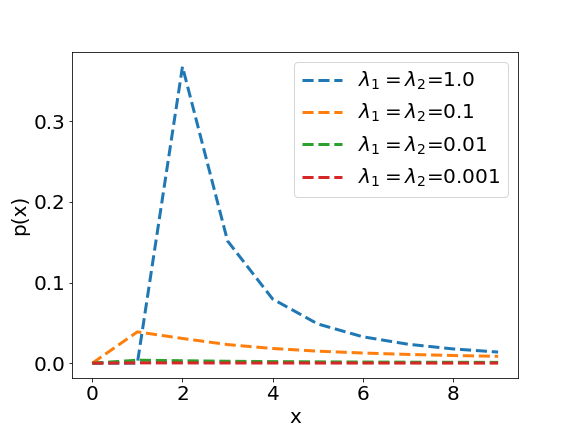
\includegraphics[width=0.6\textwidth]{plots/notebooks/invgamma.png}
\caption{Графики обратных гамма распределений для различных значений метапараметров.}
\label{fig:inv-gamma}
\end{figure}

В качестве априорного распределения для структуры $\boldsymbol{\Gamma}$ предлагается использовать произведение распределение Gumbel-Softmax~\cite{gs}:
\[
    p(\boldsymbol{\Gamma}|\mathbf{h}) = \prod_{(j,k) \in E} p(\boldsymbol{\gamma}^{j,k}|\mathbf{h}),
\]
\[
    p(\boldsymbol{\gamma}^{j,k}|\mathbf{h}) = \Gamma(K_{j,k})\lambda_{\text{temp}}^{K_{j,k}-1}\left(\sum_{p=1}^{K_{j,k}} \frac{s^{j,k}_p}{(\gamma_p^{j,k})^\lambda_{\text{temp}}}\right)^{-K_{j,k}}\left(\prod_{p=1}^{K_{j,k}} \frac{s_p}{(\gamma_p^{j,k})^{1+\lambda_{\text{temp}}}}\right),
\]
где $\mathbf{s}_{j,k} \in (0,\infty)$ --- гиперпараметр, отвечающий за смещенность плотности распределения относительно точек симплекса на $K_{j,k}$ вершинах, $\lambda_{\text{temp}}$ --- метапараметр температуры, отвечающий за концентрацию плотности вблизи вершин симплекса или в центре симплекса.

Перечислим свойства, которыми обладает распределение Gumbel-Softmax:
\begin{enumerate}
\item Реализацию $\hat{\gamma}^{j,k}_p $ случайной величины $\gamma^{j,k}$  можно породить следующим образом:
\[
    \hat{\gamma}^{j,k}_p = \frac{\text{exp}(\text{log}s^{j,k}_p+\hat{g_p})/\lambda_{\text{temp}}}{\sum_{p'=1}^{K_{j,k}}\text{exp}(\text{log}s^{j,k}_{p'}+\hat{g_{p'}})/\lambda_{\text{temp}}},
\]
где $\hat{\mathbf{g}} \sim -\text{log}\bigl(-\text{log}\mathcal{U}(0,1)\bigr).$ 

\item Свойство округления: $p(\gamma^{j,k}_{p_1} > \gamma^{j,k}_{p_2}, p_1\neq p_2) = \frac{s_p}{\sum_{p'}s_{p'}}.$

\item При устремлении температуры к нулю реализация случайной величины концентрируется на вершинах симплекса:
\[
    p(\lim_{\lambda_{\text{temp}} \to 0}  \gamma^{j,k}_{p} = 1)  = \frac{s_p}{\sum_{p'}s_{p'}}.
\]
\item При устремлении температуры к нулю плотность распределения концентрируется на вершинах симплекса:
\[
    \lim_{\lambda_{\text{temp}} \to 0}  p(\boldsymbol{\gamma}^{j,k} \in \bar{\Delta}^{K_{j,k}-1}|\mathbf{h}) = 1,
\]
где $\bar{\Delta}^{K_{j,k}-1}$ --- множество вершин симплекса на  $K_{j,k}$ вершинах.

\item При устремлении температуры к нулю плотность распределения концентрируется в центре симплекса:
\[
    \lim_{\lambda_{\text{temp}} \to \infty}  p\left(\boldsymbol{\gamma}^{j,k}_p = \frac{1}{K_{j,k}}\Bigg|\mathbf{h}\right) = 1.
\]
\end{enumerate}

Доказательства первых трех утверждений приведены в~\cite{gumbel}. Докажем утверждения 4 и 5.

\begin{proof}
TODO
\end{proof}


\begin{proof}
TODO
\end{proof}

Первое свойство Gumbel-Softmax распределения позволяет использовать репараметризацию при вычислении градиента в вариационном выводе (англ. reparametrization trick). Данный подход позволяет значительно повысить точность вычисления градиента от функций, зависящих от случайных величин~\cite{reparametrization}.
Пример распределения Gumbel-Softmax при различных параметрах представлен на Рис.~\ref{fig:gs}. Отметим, что для предлагаемой вероятностной модели можно использовать и другие распределения на симплексах, такие как распределение Дирихле или равномерное распределение. Выбор в качестве распределения на структуре произведения Gumbel-Softmax распределения обоснован выбором этого же распределения в качестве вариационного.

\begin{figure}
 \begin{minipage}[t]{.2\textwidth}
        \centering
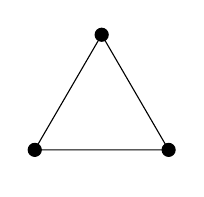
\begin{tikzpicture}[%
x={(1.7cm,0cm)},
y={(0cm,1.7cm)},
]

\coordinate (A) at (0,0); 
\coordinate (B) at (1,0) ;
\coordinate (C) at (0.5,0.86); 

%Ecken
\node[circle,scale=0.5,fill=black,draw=black](Ap) at (0,0){};
\node[circle,scale=0.5,fill=black,draw=black](Bp) at (1,0){};
\node[circle,scale=0.5,fill=black,draw=black](Cp) at (0.5,0.86){};

%Kanten
\draw[] (A)
-- (B)  node[midway, below]{}
-- (C)      node[midway, right]{}
-- (A)  node[midway, left]{};

\end{tikzpicture}
\subcaption{}
\end{minipage}
\hfill
 \begin{minipage}[t]{.2\textwidth}
   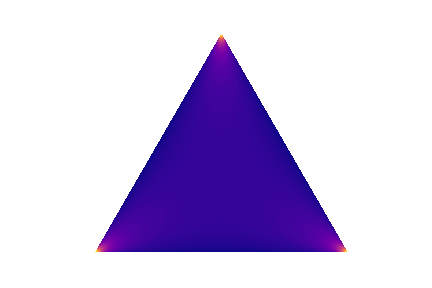
\includegraphics[width=\textwidth]{plots/notebooks/gs1.png}
\subcaption{}
\end{minipage}
\hfill
 \begin{minipage}[t]{.2\textwidth}
   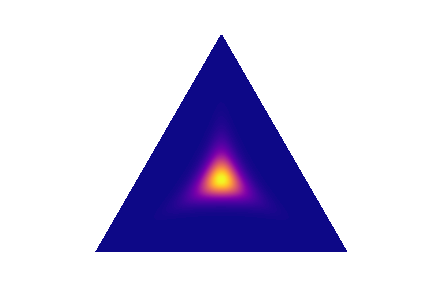
\includegraphics[width=\textwidth]{plots/notebooks/gs5.png}
\subcaption{}
\end{minipage}
\hfill
 \begin{minipage}[t]{.2\textwidth}
   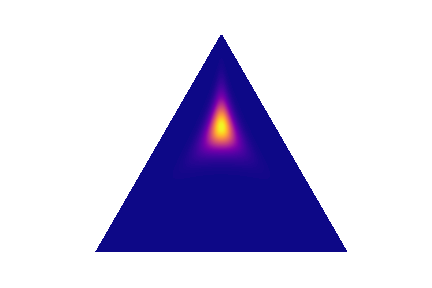
\includegraphics[width=\textwidth]{plots/notebooks/gs5_shift.png}
\subcaption{}
\end{minipage}

\caption{Пример распределения Gumbel-Softmax при различных значениях параметров: а)~$\lambda_{temp}\to0$, б)~$\lambda_{temp}=1, \mathbf{s}=[1,1,1]$, в)~$\lambda_{temp}=5, \mathbf{s}=[1,1,1]$, г)~$\lambda_{temp}=5, \mathbf{s}=[10,0.1,0.1].$}
\label{fig:gs}

\end{figure}

Таким образом, предлагаемая вероятностная модель содержит следующие компоненты:
\begin{enumerate}
\item Параметры $\mathbf{w}$ модели, распределенные нормально.
\item Структура модели $\boldsymbol{\Gamma}$ распределены по распределению Gumbel-Softmax.
\item Гиперпараметры: $\mathbf{h} = [\text{diag}(\mathbf{A}), \mathbf{s}]$, где $\mathbf{A}$ --- конкатенация матриц $\mathbf{A}^{j,k}, (j,k) \in E,$ $\mathbf{s}$ --- конкатенация параметров Gumbel-Softmax распределений $\mathbf{s}^{j,k}, (j,k) \in E$.
\item Метапараметры: $\boldsymbol{\lambda} = [\lambda_1, \lambda_2].$
\end{enumerate}

График вероятностной модели в формате плоских нотаций представлен на Рис.~\ref{fig:plate_prob}.
\begin{figure}
\centering
   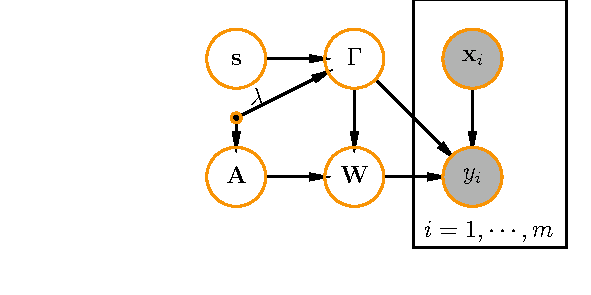
\includegraphics[width=0.5\textwidth]{plots/notebooks/simple_plate.pdf}
\caption{График предлагаемой вероятностной модели в формате плоских нотаций. Переменные обозначены белыми и серыми кругами, константы обозначены обведенными черными кругами. Наблюдаемые переменные обозначены серыми кругами.}
\label{fig:plate_prob}
\end{figure}

\section{Вариационная оценка для обоснованности вероятностной модели}
В качестве критерия выбора структуры модели предлагается использовать апостериорную вероятность гиперпараметров:
\begin{equation}
\label{eq:optimal_hyper}
    p(\mathbf{h}|\mathbf{y}, \mathbf{X}, \boldsymbol{\lambda}) \propto p(\mathbf{y}|\mathbf{X}, \mathbf{h}, \boldsymbol{\lambda}) p(\mathbf{h}|\boldsymbol{\lambda}) \to \max_{\mathbf{h} \in \mathbb{H}},
\end{equation}
где структура модели и параметры модели выбираются неявно на основе полученных значений гиперпараметров:
\[
    \boldsymbol{\Gamma} = \argmax_{\boldsymbol{\Gamma} \in \amsmathbb{\Gamma}} p(\boldsymbol{\Gamma}|\mathbf{y}, \mathbf{X}, \mathbf{h}),
\]
\[
    \mathbf{w} = \argmax_{w \in \mathbb{W}} p(\boldsymbol{w}|\mathbf{y}, \mathbf{X}, \boldsymbol{\Gamma}, \mathbf{h}).
\]

Для вычисления обоснованности $p(\mathbf{y}|\mathbf{X}, \mathbf{h}, \boldsymbol{\lambda}) = \iint_{\boldsymbol{\Gamma},\mathbf{w}}p(\mathbf{y}|\mathbf{X}, \mathbf{w}, \boldsymbol{\Gamma},\boldsymbol{\lambda})p(\mathbf{w}|\boldsymbol{\Gamma},\mathbf{h}, \boldsymbol{\lambda})p(\boldsymbol{\Gamma}|\mathbf{h}, \boldsymbol{\lambda})$ из~\eqref{eq:optimal_hyper} предлагается использовать вариационную оценку обоснованности.

\begin{theorem}
Пусть $q = q_{\mathbf{w}}q_{\boldsymbol{\Gamma}}$ --- вариационное распределение c параметрами $\boldsymbol{\theta}$, аппроксимирующее апостериорное распределение структуры и параметров:
\[
    q \approx p(\mathbf{w},\boldsymbol{\Gamma}|\mathbf{y}, \mathbf{X}, \mathbf{h}),
\]
\[
    q_{\mathbf{w}} \propto p(\mathbf{w}|\mathbf{y}, \mathbf{X},  \boldsymbol{\Gamma},\mathbf{h}),
\]
\[
    q_{\boldsymbol{\Gamma}} \propto p(\boldsymbol{\Gamma}|\mathbf{y}, \mathbf{X},  \mathbf{h}).
\]

Тогда справедлива следующая оценка:
\begin{equation}
\label{eq:full_elbo}
\text{log} p(\mathbf{y}|\mathbf{X}, \mathbf{h}, \boldsymbol{\lambda}) \geq
\end{equation}
\[
 \mathsf{E}_{\boldsymbol{\Gamma} \sim q_{\boldsymbol{\Gamma}}}\mathsf{E}_{\mathbf{w} \sim q_{\mathbf{w}}} \text{log}p(\mathbf{y}|\mathbf{w}, \boldsymbol{\Gamma}, \mathbf{X}) - D_\text{KL}\left(q_{\boldsymbol{\Gamma}}|p(\boldsymbol{\Gamma}|\mathbf{h}, \boldsymbol{\lambda})\right) - D_\text{KL}\left(q_{\mathbf{w}}|p(\mathbf{w}|\boldsymbol{\Gamma}, \mathbf{h})\right),
\]
где $D_\text{KL}\left(q_{\mathbf{w}}|p(\mathbf{w}|\boldsymbol{\Gamma}, \mathbf{h})\right)$ вычисляется по формуле условной дивергенции~\cite{TODO}:
\[
D_\text{KL}\left(q_{\mathbf{w}}|p(\mathbf{w}|\boldsymbol{\Gamma}, \mathbf{h})\right) = \mathsf{E}_{\boldsymbol{\Gamma} \sim q_{\boldsymbol{\Gamma}}} \mathsf{E}_{\mathbf{w} \sim q_{\mathbf{w}}} \frac{\text{log}q(\mathbf{w})}{\text{log}p(\mathbf{w}|\mathbf{h},\boldsymbol{\Gamma})}.
\]
\end{theorem}

\begin{proof}
TODO
\end{proof}

В качестве вариационного распределения $q_{\mathbf{w}}$ предлагается использовать нормальное распределение:
\[
    q_{\mathbf{w}} = \mathcal{N}(\boldsymbol{\mu}, \boldsymbol{\sigma}^2_q).
\]
В качестве вариационного распределения $q_{\boldsymbol{\Gamma}}$ предлагается использовать распределение Gumbel-Softmax.

Вариационными параметрами распределения $q$ являются параметры распределений $q_{\mathbf{w}}, q_{\boldsymbol{\Gamma}}$:
\[
    \boldsymbol{\theta} = [\boldsymbol{\mu}, \boldsymbol{\sigma}^2_q, \mathbf{s}_q, \theta_\text{temp}], 
\]
где $ \mathbf{s}_q, \theta_\text{temp}$ --- параметры Gumbel-Softmax распределений.

График вероятностной вариационной модели в формате плоских нотаций представлен на Рис.~\ref{fig:plate_qprob}.
\begin{figure}
\centering
   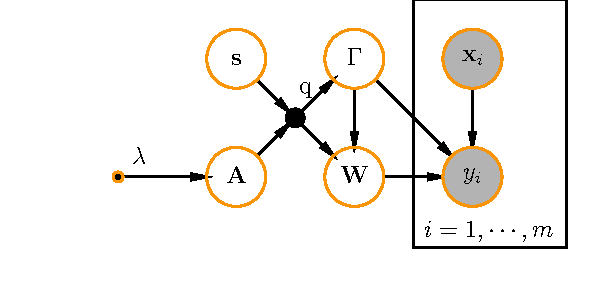
\includegraphics[width=0.5\textwidth]{plots/notebooks/plate.pdf}
\caption{График предлагаемой вероятностной вариационной модели в формате плоских нотаций. Переменные обозначены белыми и серыми кругами, константы обозначены обведенными черными кругами. Вариационное распределение обозначено черным кругом. Наблюдаемые переменные обозначены серыми кругами.}
\label{fig:plate_qprob}
\end{figure}


Для вычисления приближенного значения вариационной оценки обоснованности~\eqref{eq:full_elbo} предлагается использовать следующую формулу:
TODO.

Для анализа сложности полученной модели введем понятие \textit{параметрической сложности}. 
\begin{defin}
Параметрической сложностью  $C_p(\boldsymbol{\theta})$ модели с вариационными параметрами $\boldsymbol{\theta}$ назовем минимальную дивергенцию между вариационным и априорным распределением:
\[
C_p(\boldsymbol{\theta}) = \min_{\mathbf{h} \in \mathbb{H}} \text{D}_\text{KL}\left(q|p(\mathbf{w}, \boldsymbol{\Gamma}|\mathbf{h})\right).
\]
\end{defin}
Параметрическая сложность модели соответствует ожидаемой длине описания параметров модели при условии заданного параметрического априорного распределения~\cite{hinton_mdl}.

Одним из критериев удаления неинформативных параметров в вероятностных моделях является вариационная плотность~\cite{nips}: отношение вариационной плотности параметров в моде распределения к вариационной плотности параметра в нуле:
\[
    \rho(q_{\mathbf{w}}) = \frac{q(\mu)}{q(0)} = \text{exp}\left(\frac{-2\sigma_q^2}{\mu^2}\right).
\]

Сформулируем и докажеми теорему о связи относительной плотности и параметрической сложности модели:
\begin{theorem}
Пусть $\boldsymbol{\theta}_1,\boldsymbol{\theta}_2,\dots$ --- бесконечная последовательность векторов вариационных параметров, такая что $\lim_{i \to \infty}C_p(\boldsymbol{\theta}_i) = 0$. Тогда относительная плотность вариационных параметров данной последовательности стремится к единице:
\[
    \lim_{i\to\infty} \boldsymbol{\rho}(q) = 1.
\]
\end{theorem}
Теорема утверждает, что при устремлении параметрической сложности моделей к нулю, параметры модели станоятся неинформативными и подлежащими удалению.

\textbf{Обобщающая задача}


\textbf{Обобщающая задача: критерии не являются обобщающими}

\textbf{Обобщающая задача: предлагаемая}


\textbf{Обобщающая задача: иллюстрация перебора}

\textbf{Обобщающая задача: переформулировка через градиент}

\textbf{Обобщающая задача: адекватность задачи}

\textbf{Обобщающая задача: свойства коэффициентов}

\textbf{Решение задачи}

\textbf{Эксперимент: пример 1}

\textbf{Эксперимент: пример 2}
































\iffalse


\section{Постановка задачи выбора структуры модели}
Задана выборка \begin{equation}\label{eq:dataset}\mathfrak{D} = \{(\mathbf{x}_i,y_i)\}, i = 1,\dots,m,\end{equation} состоящая из множества пар <<объект-метка>> $$\mathbf{x}_i \in \mathbf{X} \subset \mathbb{R}^n, \quad {y}_i \in \mathbf{y} \subset \mathbb{Y}.$$ Метка ${y}$  объекта $\mathbf{x}$ принадлежит либо множеству: ${y} \in \mathbb{Y} = \{1, \dots, Z\}$ в случае задачи классификации, где $Z$ --- число классов, либо некоторому подмножеству вещественных чисел ${y} \in \mathbb{Y}  \subseteq \mathbb{R}$ в случае задачи регрессии. Положим, что пары объект $(\mathbf{x}, y)$ являются реализацией некоторой случайно величины и порождены независимо.

Пусть задано семейство моделей глубокого обучения $\mathfrak{F}$.
Пусть значения каждого структурного параметра $\boldsymbol{\gamma}^{i,j}$ лежат на симплексе $\Delta^{K^{i,j}-1}$.
Пусть для каждого структурного параметра $\boldsymbol{\gamma}^{i,j} \in \boldsymbol{\Gamma}$ определено параметрическое априорное распределение $p(\boldsymbol{\gamma}^{i,j}), \mathbf{m}^{i,j}, \text{c}_{\text{temp}}),$ где где $\mathbf{m}^{i,j}$ --- параметр средних,  $c_{\text{temp}}$ --- температура (или концентрация) распределения.
Перечислим свойства, которыми должно обладать данное распределение:
\begin{enumerate}
\item $p(\boldsymbol{\gamma}^{i.j})$ является непрерывным на симплексе $\Delta^{K^{i,j}-1}$.
\item При устремлении температуры к бесконечности распределение сходится к равномерному: $\lim_{c_{\text{temp}} \to \infty} = p(\boldsymbol{\gamma}^{i,j}), \mathbf{m}^{i,j}, \text{c}_{\text{temp}}) = \mathcal{U}(\Delta^{K^{i,j}-1}).$
\item При устремлении температуры к нулю распределение сходится к сингулярному распределению следующего вида:
$\lim_{c_{\text{temp}} \to 0}  p(\gamma^{i,j}_k) = m^{i,j}_k.$
\end{enumerate}

\begin{utv}
Перечисленными свойствами обладают распределения Дирихле и Гумбель-софтмакс.
\end{utv}

Обозначим через $S$ сюрьективное отношение между параметром модели $w \in \mathbf{w}$ и весами $\boldsymbol{\gamma}$ базовых функцией $\mathbf{g}$, определенное по следующему правилу:\\
\textit{Если $w \in \mathbf{w}$ является параметром функции $\mathbf{g}^{i,j}_k$, где $(i,j) \in E$, то $S(w) = \gamma^{i,j}_k$.}\\
Априорное распределение параметров  зададим следующим образом:
\[
    \mathbf{w} \sim \mathcal{N}\left(\mathbf{0}, \mathbf{A}^{-1} \otimes S(\mathbf{w})\right).
\]
где $\mathbf{A}$ --- диагональная матрица с положительными элементами на диагонали.
Пусть также определено правдоподобие выборки $p(\mathbf{y}|\mathbf{X}, \mathbf{w}, \boldsymbol{\Gamma}).$\\

Задача выбора структуры модели предполагает поиск значений гиперпараметров модели $\mathbf{A}, \mathbf{m}$ доставляющих максимум правдоподобия модели:
\begin{equation}
\label{eq:evidence_optim}
    \argmax_{\mathbf{A}, \mathbf{m}}  p(\mathbf{y}|\mathbf{X},\mathbf{A},\mathbf{m}, {c_\text{temp}}),
\end{equation}

а также соответствующие параметры и структуру модели:
\begin{equation}
\label{eq:params_optim}
    \argmax_{\mathbf{w}, \boldsymbol{\Gamma}}  p(\mathbf{w}, \boldsymbol{\Gamma}|\mathbf{X},\mathbf{y}, \mathbf{A}, \mathbf{m}, {c_\text{temp}}).
\end{equation}

 \begin{figure}[H]
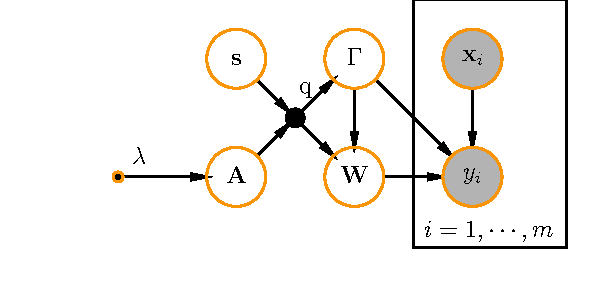
\includegraphics[width=\textwidth]{./plots/notebooks/plate.pdf}
\caption{Plate notation}
\end{figure}

TODO: схема\\.


Для определения возможных значений структуры $\boldsymbol{\Gamma}$ введем следующие обозначения.
Обозначим через $\Delta(\boldsymbol{\Gamma})$ множество точек, лежащих внутри произведения симплексов, определенных на структурных параметрах
$$
\Delta(\boldsymbol{\Gamma}) =  \prod{i,j \in E}\Delta^{K^{i,j}-1}.
$$
Обозначим через $\bar{\Delta}(\boldsymbol{\Gamma})$ только те точки $\Delta(\boldsymbol{\Gamma})$, которые принадлежат вершинам соответствующих симплексов.


Докажем теорему об оптимальности решения задачи~\eqref{eq:params_optim}, лежащего на вершинах симплексов $\times_{(i,j) \in E} \Delta^{K^{i,j}-1}$. 


\textbf{Теорема.} \\
Пусть $\boldsymbol{\Gamma}_1$ и $\boldsymbol{\Gamma}_2$ --- реализации $\boldsymbol{\Gamma}$, такие что:
\begin{itemize}
\item $\boldsymbol{\Gamma}_1 \in \bar{\Delta}(\boldsymbol{\Gamma})$.
\item $\boldsymbol{\Gamma}_2 \not \in \bar{\Delta}(\boldsymbol{\Gamma})$.
\end{itemize} 
Тогда для любых положительно определенных матриц $\mathbf{A}_1$ и $\mathbf{A}_2$ и векторов $\mathbf{m}_1, \mathbf{m}_2, \text{min}(\mathbf{m}_1)>0$ справедлива следующее отношение апостериорных вероятностей:
$$\lim_{c_\text{temp} \to 0} \frac{p(\boldsymbol{\Gamma}_2, \mathbf{w}_2|\mathbf{y},  \mathbf{X},\mathbf{A}_1,\mathbf{m}_2, {c_\text{temp}})}{p(\boldsymbol{\Gamma}_1,  \mathbf{w}|\mathbf{y}, \mathbf{X},\mathbf{A}_1,\mathbf{m}_1, {c_\text{temp}})} = \infty.$$

\textbf{Доказательство}.\\
По свойству априорного распределения структурных параметров
$$p(\lim_{c_{\text{temp}} \to 0} {\gamma}^{i,j}_k  = 1) = {m}^{i,j}_k.$$

Тогда:
$$p(\lim_{c_{\text{temp}} \to 0} \boldsymbol{\gamma}^{i,j} \in \bar{\Delta}^{K^{i,j}}) = 1.$$

Тогда апостериорная вероятность $\boldsymbol{\Gamma}:$ в пределе равняется нулю, если структура не лежит на произведении вершин симплекса.

$$p(\boldsymbol{\Gamma}_2, \mathbf{w}+2|\mathbf{y}, \mathbf{X},\mathbf{A}_2,\mathbf{m}_2, {c_\text{temp}}) \propto p(\boldsymbol{\Gamma}) p(\mathbf{y} |\boldsymbol{\Gamma},   \mathbf{w}, \mathbf{X},\mathbf{A}_1,\mathbf{m}) \to 0,$$
$$p(\boldsymbol{\Gamma}_1,  \mathbf{w}_1|\mathbf{y}, \mathbf{w}, \mathbf{X},\mathbf{A}_1,\mathbf{m}_1, {c_\text{temp}}) \propto p(\boldsymbol{\Gamma}) p(\mathbf{y} |\boldsymbol{\Gamma},  \mathbf{X},\mathbf{A}_1,\mathbf{m}) \to C,$$
где $C$ --- константа, большая нуля, т.к. $ \text{min}(\mathbf{m}_1)>0$.
что и требовалось доказать.

\textbf{Решение задачи с помощью вариационного вывода}\\
В общем виде получение значения интеграла~\eqref{eq:evidence} является вычислительно сложной процедурой. В качестве приближенного значения интеграла используется вариационную верхнюю оценку правдоподобия модели. 

Будем приближать неизвестное апостериорное распределение апостериорные распределение параметрическим распределением $q$ с параметрами $\boldsymbol{\theta}$.
Разница между верхней оценкой~\eqref{eq:elbo} и правдоподобием модели~\eqref{eq:evidence} определяется дивергенцией между вариацоинным распределение $q$ и апостериорным распределением $p(\mathbf{w}, \boldsymbol{\Gamma}|\mathbf{y}, \mathbf{X}, \mathbf{A},\mathbf{m}, c_{\text{temp}})$. 

Зададим вариацонное распределение $q$ следующим образом. 
Факторизуем $q$ на два распределения: 
$$q = q_{\mathbf{w}}q_{\boldsymbol{\Gamma}}:
q_{\mathbf{w}} \sim \mathcal{N}(\boldsymbol{\mu}_q, \mathbf{A}^{-1}_q), \quad q_{\boldsymbol{\Gamma}} = \prod_{(i,j) \in E} q_\gamma^{i,j}, \quad q_\gamma \sim \mathcal{GS}( \mathbf{m}_q^{i,j}, c_q).$$
Обозначим за $\mathbf{m}_q$ конкатенацию всех векторов средних  $\mathbf{m}_q^{i,j}$.

Для получения значения $\text{log}_q {p}(\mathbf{y}|\mathbf{X},\mathbf{A},\mathbf{m}, c_{\text{temp}})$ использубися следующие методы сэмплирования:
$$
    \mathsf{E}_{q}\text{log} p(\mathbf{y}|\mathbf{X},\mathbf{w}, \boldsymbol{\Gamma}, \mathbf{A},\mathbf{m}, c_{\text{temp}}) \approx \frac{1}{N}\sum_{u =1}^{N} \text{log} p(\mathbf{y}|\mathbf{X},\hat{\mathbf{w}}_u, \hat{\boldsymbol{\Gamma}}_u, \mathbf{A},\mathbf{m}, c_{\text{temp}}),
$$
$$
   {D_{KL}}(q||p(\mathbf{w}, \boldsymbol{\Gamma}| \mathbf{A},\mathbf{m}, c_{\text{temp}}) = {D_{KL}}(q_{\boldsymbol{\Gamma}}||p(\boldsymbol{\Gamma}| \mathbf{m}, c_{\text{temp}}) + {D_{KL}}(q_{\mathbf{w}||p(\mathbf{w}|\mathbf{A}}) \approx
$$
$$
    \frac{1}{N}\sum_{u=1}^N (\text{log}~q_{\boldsymbol{\Gamma}}(\hat{\boldsymbol{\Gamma}_u}) - \text{log}p(\hat{\boldsymbol{\Gamma}_u}) + 0.5(\text{tr}(\hat{\mathbf{S}}_u(\mathbf{w})\mathbf{A}\mathbf{A}_q^{-1}) + $$
$$+\boldsymbol{\mu}^{\text{T}}\hat{\mathbf{S}}_u(\mathbf{w})\mathbf{A}\boldsymbol{\mu} - |\mathbf{w}| + \text{log det}\hat{\mathbf{S}}_u(\mathbf{w})\mathbf{A} -  \text{log det}\mathbf{A}_q )),
$$
где $N$ --- количество реализаций случайных величин, $\hat{\boldsymbol{\Gamma}}_u, \hat{\mathbf{w}}_u$ --- реализации случайных величин, $\hat{S_u}(\mathbf{w})$ --- соответствие между параметрами и реализацией весов базовых функций.

Сэмплирование происходит следующим образом:
$$
    \hat{\mathbf{w}} = \boldsymbol{\mu} + \varepsilon\mathbf{A}_q, \quad \varepsilon \in \mathcal{N}(\mathbf{0}, \mathbf{1}),
$$
$$
    \hat{\boldsymbol{\gamma}}_k = \frac{\text{exp}((\text{log}{m}_k + a_k) / c )}{\sum_{i=1}^K (\text{log}{m}_i + a_i) / c )}, \quad \mathbf{a} \in -\text{log}(\text{log}(\mathcal{U}(0, 1)^K).
$$
Численную оценку, полученную описанным выше способом будет обозначать как 
$$\hat{\text{log}_q} {p}(\mathbf{y}|\mathbf{X},\mathbf{A},\mathbf{m}, c_{\text{temp}}) = \hat{\mathsf{E}_{q}}\text{log} p(\mathbf{y}|\mathbf{X},\mathbf{w}, \boldsymbol{\Gamma}, \mathbf{A},\mathbf{m}, c_{\text{temp}}) - \hat{D_{KL}}(q||p(\mathbf{w}, \boldsymbol{\Gamma}| \mathbf{A},\mathbf{m}, c_{\text{temp}})).$$

TODO: plate-notation.


Докажем теорему о дискретности задачи оптимизации вариационной оценки в предельном случае.\\
\textbf{Теорема.} 
Пусть $c = c_\text{temp}$.
Для любых значений ковариационных матриц $\mathbf{A}, \mathbf{A}_q$, любого вектора $\boldsymbol{\mu}_q$ существуют такие точки $\mathbf{m}_q^1 \in \times_{(i,j) \in E} \bar{\Delta}^{K^{i,j}-1}, \mathbf{m}^1 \in \times_{(i,j) \in E} \bar{\Delta}^{K^{i,j}-1}$ на вершинах симплексов структуры $\boldsymbol{\Gamma}$,  что для любой точки  $\mathbf{m}_q^2  \in \times_{(i,j) \in E} \Delta^{K^{i,j}-1}$ и $\mathbf{m}^2  \in \times_{(i,j) \in E} \Delta^{K^{i,j}-1}$ внутри симплексов справедливо выражение:
$$\lim_{c_\text{temp} \to 0}\frac{\text{log}\hat{{p}}_{q_{\mathbf{w}}q^2_{\boldsymbol{\Gamma}}}(\mathbf{y}|\mathbf{X})}{\text{log}\hat{{p}}_{q_{\mathbf{w}}q_{\boldsymbol{\Gamma}}}(\mathbf{y}|\mathbf{X})} \geq 1,\text{\quad где}
q_{\boldsymbol{\Gamma}}^1 = \max_{c} q_{\boldsymbol{\Gamma}}( \mathbf{m}_q^1, c).$$

\textbf{Доказательство.}
По свойству предельного распределения $\mathcal{GS}$ задача сводится к задаче с сингулярным распределением на структурах.
Расписав $\text{log}_q {p}(\mathbf{y}|\mathbf{X},\mathbf{A},\mathbf{m}, c_{\text{temp}})$ через двойную сумму находим максимальный элемент.


\section{Обобщенная постановка задачи}
Определим основные величины, которые характеризуют сложность модели. \\

\textbf{Определение} Параметрической сложностью $C_{\mathbf{w}}$ модели назовем наименьшую дивергенцию вариационного распределения при условии заданного априорного распределения параметров:
\[
    C_{\mathbf{w}} = \argmin_\mathbf{A} D_\text{KL}\left(q|p(\mathbf{w}, \boldsymbol{\Gamma}|\mathbf{A}, \mathbf{m}, {\boldsymbol{c}_\text{temp}})\right).
\]

\textbf{Определение} Структурной сложностью $C_{\boldsymbol{\Gamma}}$ модели назовем энтропию распределения структуры:
\[
    C_{\boldsymbol{\Gamma}} = -\mathsf{E}_{q_{\boldsymbol{\Gamma}}} \text{log}q_{\boldsymbol{\Gamma}},
\]
где $q_{\boldsymbol{\Gamma}}$ --- вариационное распределение структуры модели.

В силу многоэкстремальности задачи~\eqref{eq:optim}, оптимизация параметров вариационных распределений $\boldsymbol{\theta}$ и априорных распределений $\mathbf{h}$ должна позволять не только находить локальный оптимум задачи~\eqref{eq:optim}, но и использовать ряд эвристических алгоритмов, таких как снижение и наращивание сложности модели. 
Сформулируем основные требования к оптимизационной задаче и оптимизируемым функционалам:
\begin{enumerate}
\item Оптимизируемые функции $L,Q$ должны быть дифференцируемы.
\item Распределение параметров модели, являющееся решением задачи оптимизации должно доставлять максимум апостериорной вероятности в некоторой окрестности.
\item Степень регуляризации структуры $\boldsymbol{\Gamma}$ и параметров $\mathbf{w}$ должна быть контролируемой.
\item Решение задачи оптимизации должно являться локально-оптимальным для вариационной оценки~\eqref{eq:elbo}.
\item Оптимизация должна позволять варьировать параметрическую сложность модели $C_{\mathbf{w}}$.
\item Оптимизация должна позволять варьировать структурную сложность ${\boldsymbol{\Gamma}}$ модели.
\item Оптимизация должна позволять проводить полный перебор структуры $\boldsymbol{\Gamma}$.
\end{enumerate}


Сформулируем задачу как двухуровневую задачу оптимизации. обозначим через  $\boldsymbol{\theta}$ оптимизируемые на первом уровне величины. обозначим через $\mathbf{h}$ величины, оптимизируемые на втором уровне.
Положим $\boldsymbol{\theta}$ равным параметрам распределений $q_{\mathbf{w}}, q_{\boldsymbol{\Gamma}}: \boldsymbol{\theta} = [\boldsymbol{\mu}_q, \mathbf{A}_q, \mathbf{m}_q, c]^\text{T}$.  
Положим $\mathbf{h} = [\mathbf{A}, \mathbf{m}].$

обозначим через $L$ функцию потерь:
\begin{equation}
    L = c_{\text{reg}}{\mathsf{E}_{q}}\text{log} p(\mathbf{y}|\mathbf{X},\mathbf{w}, \boldsymbol{\Gamma}, \mathbf{A},\mathbf{m}, c_{\text{temp}})
 - {D_{KL}}(q_{\boldsymbol{\Gamma}}||p(\boldsymbol{\Gamma})) - {D_{KL}}(q_{\mathbf{w}}||p(\mathbf{w})),
\end{equation}
где $c_{\text{reg}}$ --- коэффициент регуляризации регуляризации структуры $\boldsymbol{\Gamma}$ и параметров $\mathbf{w}$ априорным распределением.

\textbf{Лемма.}  Пусть $\mathbf{A}_q$ фиксирована и близка к нулю, $c_{\text{reg}} =1$.  Тогда максимизация $L$ эквивалентна оптимизации апостериорной вероятности параметров при $c \to 0$.\\
\textbf{Доказательство.} 
$L = \mathsf{E}_{q}\text{log} p(\mathbf{y}|\mathbf{X},\mathbf{w}, \boldsymbol{\Gamma}, \mathbf{A},\mathbf{m}, c_{\text{temp}}) - {D_{KL}}(q||p(\mathbf{w}, \boldsymbol{\Gamma}| \mathbf{A},\mathbf{m}, c_{\text{temp}})).$
Полагая ковариационную матрицу близкой к нулю $$ \mathsf{E}_{q}\text{log} p(\mathbf{y}|\mathbf{X},\mathbf{w}, \boldsymbol{\Gamma}, \mathbf{A},\mathbf{m}, c_{\text{temp}}) \approx \text{log} p(\mathbf{y}|\mathbf{X},\boldsymbol{\mu}_q, \boldsymbol{\Gamma}, \mathbf{A},\mathbf{m}, c_{\text{temp}})$$.

$$
   {D_{KL}}(q||p(\mathbf{w}, \boldsymbol{\Gamma}| \mathbf{A},\mathbf{m}, c_{\text{temp}}) = 
$$
$$
    \frac{1}{N}\sum_{u=1}^N (\text{log}~q_{\boldsymbol{\Gamma}}(\hat{\boldsymbol{\Gamma}_u}) - \text{log}p(\hat{\boldsymbol{\Gamma}_u}) + 0.5(\boldsymbol{\mu}^{\text{T}}\hat{\mathbf{S}}_u(\mathbf{w})\mathbf{A}\boldsymbol{\mu} - |\mathbf{w}| + \text{log det}\hat{\mathbf{S}}_u(\mathbf{w})\mathbf{A}).
$$

Следующая теорема говорит о том, что варьируя $c_{\text{reg}}$ мы проводим оптимизацию, ассимптотически аналогичную оптимизации выборки из того же распределения, но другой мощности.

\textbf{Теорема}. Пусть $c_{\text{reg}} > 0$, $c_{\text{reg}} m \in \mathbb{N}.$
Тогда функция $L$ сходится почти наверно к вариационной нижней оценке правдоподобия для произвольной подвыборки  $\mathfrak{D}$ 
мощностью $m_0 = \frac{m}{c_{\text{reg}}}$, поделенной на данную константу.\\

\textbf{Доказательство}. Рассмотрим произвольную подвыборку $\hat{\mathfrak{D}}$ мощностью $m_0$. Нижняя оценка правдоподобия модели для подвыборки имеет вид:
\[
 \mathsf{E}_{q_w,q_\gamma}\text{log} p(\hat{\mathbf{y}}|\hat{\mathbf{X}},\mathbf{w}, \boldsymbol{\Gamma}, \mathbf{A},\mathbf{m}, c) - {D_{KL}}(q_\gamma||p(\boldsymbol{\Gamma})) - {D_{KL}}(q_{w}||p(\mathbf{w})).
\]

\[
\text{log} p(\hat{\mathbf{y}}|\hat{\mathbf{X}},\mathbf{w}, \boldsymbol{\Gamma}, \mathbf{A},\mathbf{m}, c) = \sum_i \text{log} p(\hat{\mathbf{y}_i}|\hat{\mathbf{x}_i},\mathbf{w}, \boldsymbol{\Gamma}, \mathbf{A},\mathbf{m}, c) \to^{\text{п.н.}}_{m \to \infty} m_0\mathsf{E}\text{log} p(\mathbf{y}|{\mathbf{x}},\mathbf{w}, \boldsymbol{\Gamma}, \mathbf{A},\mathbf{m}, c).
\]

Таким образом, ассимптотическая формула вариационной нижней оценки правдоподобия для подвыборки мощностью $m_0$ выглядит следующим образом:
\[
m_0\mathsf{E}\text{log} p(\mathbf{y}|{\mathbf{x}},\mathbf{w}, \boldsymbol{\Gamma}, \mathbf{A},\mathbf{m}, c) - {D_{KL}}(q_\gamma||p(\boldsymbol{\Gamma})) - {D_{KL}}(q_{w}||p(\mathbf{w})).
\]
Домножив на выражение на $\frac{m}{m_0}$ получаем ассимптотику для $L$, что и требовалось доказать.

Пусть $Q$ --- валидационная функция:
\[
Q = {c_\text{train}\mathsf{E}_q \text{log}~{p(\mathbf{y} | \mathbf{X}, \mathbf{w}, \boldsymbol{\Gamma}. \mathbf{A}^{-1}, c_{\text{prior}})}}
 - {c_\text{prior}\text{D}_{KL}(p(\mathbf{w}, \boldsymbol{\Gamma} |\mathbf{A}^{-1}, \mathbf{m}, c_{\text{temp}}) || q(\mathbf{w}, \boldsymbol{\Gamma}))} -\]
\[
{c_{\text{comb}}\sum_{p' \in \mathbf{P}} \text{D}_{KL}(\boldsymbol{\Gamma} | p')} \to \max, 
\]
где $\mathbf{P}$ --- множество (возможно пустое) распределений на структуре модели, $c_\text{prior}$ --- коэффициент регуляризации параметрической сложности модели, 
$c_{\text{comb}}$ --- коэффициент перебора.

Сформулируем задачу поиска оптимальной модели как двухуровневую задачу.
\begin{equation}
\label{eq:optim}
	\hat{\mathbf{h}} = \argmax_{\mathbf{h} \in \mathbb{R}^h} Q( T^\eta(\boldsymbol{\theta}_0, \mathbf{h})),
\end{equation}
где $T$ --- оператор оптимизации, решающий задачу оптимизации:
\[
    L(T^\eta(\boldsymbol{\theta}_0, \mathbf{h})) \to \max.
\]


\textbf{Теорема}. Пусть $D_{KL}(q_w|p(\mathbf{w}|\mathbf{y}, \mathbf{X}, \mathbf{A},\mathbf{m}, c)) = 0, D_{KL}(q_\gamma|p(\boldsymbol{\Gamma}|\mathbf{y}, \mathbf{X}, \mathbf{A},\mathbf{m}, c)) = 0$, пусть $c_{\text{prior}} = 1, c_{\text{reg}} = 1, c_{\text{comb}} = 0$. Тогда оптимизация $\eqref{eq:optim}$ эквивалентна оптимизации $\eqref{eq:evidence}$.\\~\\
\textbf{Доказательство.} При соблюдении условий теоремы оптимизация вариационной оценки эквивалента оптимизации правдоподобия модели.
При $c_{\text{prior}} = 1, c_{\text{reg}} = 1, c_{\text{comb}} = 0$, функция $Q$ становится равной вариационной нижней оценке. 
Таким образом, двухуровневая оптимизация становится эквивалентной оптимизации правдоподобия модели по $\mathbf{A},\mathbf{m}$, что и требовалось доказать.

\section{Анализ предложенного метода выбора структуры модели}

обозначим через $F(c_{\text{reg}}, c_{\text{train}}, c_{\text{prior}}, c_{\text{comb}}, \mathbf{P}, c_{\text{temp}})$ множество экстремумов функции $L$ при решении задачи двухуровневой оптимизации.


\textbf{Теорема.}  
Пусть $\mathbf{f}_1 \in F(1, 1, c_{\text{prior}}^1, 0, \varnothing,  c_{\text{temp}} ), \mathbf{f}_2 \in F(1, 1, c_{\text{prior}}^2, 0, \varnothing,  c_{\text{temp}})$, $c_{\text{prior}}^1 < c_{\text{prior}}^2$.\\
Пусть вариационные параметры моделей $\mathbf{f}_1$ и $\mathbf{f}_2$ лежат в области $\mathsf{U}$, в которой соответствующие функции $L$ и $Q$ являются локально-выпуклыми.\\ 
Тогда модель $\mathbf{f}_1$ имеет параметрическую сложность, не меньшую чем у $\mathbf{f}_2$.
\[
    C_\text{param}(\mathbf{f}_1) \geq C_\text{param}(\mathbf{f}_2).
\]

\textbf{Доказательство.}
обозначим через $q^1, q^2$ --- вариационные распределения моделей $\mathbf{f}_1, \mathbf{f}_2$, 
$p^1, p^2$ --- априорные распределения моделей.
 
 Отсюда справедливы следующие неравенства (по единственности точек экстремума $L,Q$):
\[
    \mathsf{E}_{q^1}\text{log} p(\mathbf{y}|\mathbf{X},\mathbf{w}, \boldsymbol{\Gamma}, \mathbf{A},\mathbf{m}, c) - c_{\text{prior}}^1  D_\text{KL}(q^1||p^1)  -  \mathsf{E}_{q^2}\text{log} p(\mathbf{y}|\mathbf{X},\mathbf{w}, \boldsymbol{\Gamma}, \mathbf{A},\mathbf{m}, c) + c_{\text{prior}}^1  D_\text{KL}(q^2||p^2) \geq 0,
\]
\[
    \mathsf{E}_{q^2}\text{log} p(\mathbf{y}|\mathbf{X},\mathbf{w}, \boldsymbol{\Gamma}, \mathbf{A},\mathbf{m}, c) - c_{\text{prior}}^2  D_\text{KL}(q^2||p^2)  -  \mathsf{E}_{q^1}\text{log} p(\mathbf{y}|\mathbf{X},\mathbf{w}, \boldsymbol{\Gamma}, \mathbf{A},\mathbf{m}, c) + c_{\text{prior}}^2  D_\text{KL}(q^1||p^1) \geq 0.
\]

Складывая неравенства получим:
\[
    D_\text{KL}(q^1||p^1) \geq D_\text{KL}(q^2||p^2),
\]
\[
    \mathsf{E}_{q^2}\text{log} p(\mathbf{y}|\mathbf{X},\mathbf{w}, \boldsymbol{\Gamma}, \mathbf{A},\mathbf{m}, c)  \leq
\[ \mathsf{E}_{q^1}\text{log} p(\mathbf{y}|\mathbf{X},\mathbf{w}, \boldsymbol{\Gamma}, \mathbf{A},\mathbf{m}, c) .
\]

С учетом полученных неравенств распишем доказываемое утверждение:
\[
    \max_p \left(-D_\text{KL}(q^1||p)\right) - \max_{p} \left(-D_\text{KL}(q^2||p^2)\right) = 
\]
\[ \max_p  \left(-c_{\text{prior}}^2 D_\text{KL}(q^1||p) +\mathsf{E}_{q^1}\text{log} p(\mathbf{y}|\mathbf{X},\mathbf{w}, \boldsymbol{\Gamma}, \mathbf{A},\mathbf{m}, c) - \mathsf{E}_{q^1}\text{log} p(\mathbf{y}|\mathbf{X},\mathbf{w}, \boldsymbol{\Gamma}, \mathbf{A},\mathbf{m}, c) \right) -
\]
\[  - \max_{p} \left(-c_{\text{prior}}^2 D_\text{KL}(q^2||p)  + \mathsf{E}_{q^2}\text{log} p(\mathbf{y}|\mathbf{X},\mathbf{w}, \boldsymbol{\Gamma}, \mathbf{A},\mathbf{m}, c) +\mathsf{E}_{q^2}\text{log} p(\mathbf{y}|\mathbf{X},\mathbf{w}, \boldsymbol{\Gamma}, \mathbf{A},\mathbf{m}, c)  \right)    \leq 0,  
\]
что и т.д.
\clearpage

\textbf{Теорема.}
Пусть $\mathbf{f} \in F(1, 1, c_{\text{prior}}, 0, \varnothing,  c_{\text{temp}} )$.
При устремлении $ c_{\text{prior}}$ к бесконечности параметрическая сложность модели $\mathbf{f}$ устремляется к нулю (или сущесвтует?):
\[
    \lim_{c_{\text{prior}} \to \infty} C_{\text{param}}(\mathbf{f}) = 0.
\]

\textbf{Доказательство}\\
В пределе: $Q = D_{KL}.$\\
Минимум достигается при совпадении параметров распределений: $mu = 0$.\\
Докажем существование решения $L$, которое удовлетворяет этому.\\
Рассмотрим значение $L$ при $A \to 0$. Два случая: либо конечное значение, либо бесконечное.\\
Таким образом, калибруя $A$ получаем значения, близкие к нулю. \\
Рассмотрим последовательность. Тогда lim inf ->0.\\
Доказано. 


\textbf{Теорема}
Пусть для каждого ребра $(i,j)$ семейства моделей $\mathfrak{F}$ априорное распределение $$p(\boldsymbol{\gamma}_{i,j}) =  \lim_{c_{\text{temp}} \to 0} \mathcal{GS}(c_{\text{temp}}).$$
Пусть $c_{\text{reg}} >0, c_{\text{train}} >0, c_{\text{prior}}>0$.
Пусть $\mathbf{f} \in F(c_{\text{reg}}, c_{\text{train}}, c_{\text{prior}}, 0, \varnothing, c_{\text{temp}})$.
Тогда структурная сложность модели $\mathbf{f}$ равняется нулю.
\[
    C_\text{struct}(\mathbf{f}) = 0.
\]
    
\textbf{Доказательство}
1. Доказываем, что гипер-концентрация будет лежать на вершине\\
2. У нас получается, что $D_{KL}$ будет конечным только в случае совпадения.(???)
3. Итого, получили.

\textbf{Теорема}
Пусть $\mathbf{f}_1 \in F(c_{\text{reg}}, c_{\text{train}},  c_{\text{prior}}, 0, \varnothing,  c^1_{\text{temp}}), \mathbf{f}_2   \in \lim_{c^2_{\text{temp}} \to \infty} F(c_{\text{reg}}, c_{\text{train}},  c_{\text{prior}}, 0, \varnothing,  c^2_{\text{temp}})$.
Пусть вариационные параметры моделей $f_1$ и $f_2$ лежат в области $U$, в которой соответствующие функции $L$ и $Q$ являются локально-выпуклыми. 
Тогда разница структурных сложностей моделей ограничена выражением:
\[
    C_\text{struct}(\mathbf{f}_1)  - C_\text{struct}(\mathbf{f}_2) \leq {\mathsf{E}_q^1 \text{log}~{p(\mathbf{y} | \mathbf{X}, \mathbf{w}, \boldsymbol{\Gamma}. \mathbf{A}^{-1}, c^1_{\text{temp}})}} - {\mathsf{E}_q^2 \text{log}~{p(\mathbf{y} | \mathbf{X}, \mathbf{w}, \boldsymbol{\Gamma}, \mathbf{A}^{-1})}}.
\]

\textbf{Доказательство}
0. Доказываем равномерную сходимость.\\
1. расписываем неравенства вида: $L_1 - DKL(q_1|p1) <L_2 - DKL(q_2|p1)$\\
2. Замечаем, что при стремлении к бесконечности гумбель превращается в равномерное\\
3. выражаем все в равномерном\\
4. замечаем, что $D_KL = Entropy + const$ для равномерного



\textbf{Утверждение (очень предварительно).} Изменение $c$ позволяет избежать ухода в локальный минимум. 

\textbf{Утверждение (очень предварительно).} Изменение $c_2$ позволяет избежать ухода в локальный минимум.

\textbf{Утверждение (очень предварительно).} Взаимосвязь структуры и параметров в prior позволяет получить <<хорошие>> модели.

\textbf{Утверждение (предварительно).} Пусть $c_1 = c_2 = c_3 = 0$. Пусть $q_w \sim \mathcal{N}(\mathbf{0}, \sigma), \sigma \sim 0$. 
Тогда оптимизация эквивалентна обычной оптимизации параметров с $l_2$ - регуляризацией.

\fi
